\documentclass{../../templates/lkx_pset}

\title{Astron 140 Problem Set 6}
\author{Lev Kruglyak}
\due{October 22, 2024}

\usepackage{mdframed}


\usepackage[T1]{fontenc}
\RequirePackage{mlmodern}


\mdfdefinestyle{answer}{%
	linecolor=black,
	outerlinewidth=2pt,
	%roundcorner=20pt,
	innertopmargin=4pt,
	innerbottommargin=4pt,
	innerrightmargin=4pt,
	innerleftmargin=4pt,
	leftmargin = 4pt,
	rightmargin = 4pt
	%backgroundcolor=gray!50!white}
}

\newenvironment{answerbox}{
	\begin{mdframed}[style=answer,nobreak=true,userdefinedwidth=30em]}{\end{mdframed}}

\usepackage{siunitx}
\providecommand{\unitsi}[1]{\qty[per-mode = symbol]{#1}{}}
\providecommand{\mpssi}[1]{\qty[per-mode = symbol]{#1}{\m\per\s}}
\providecommand{\mpsssi}[1]{\qty[per-mode = symbol]{#1}{\m\per\s^2}}
\providecommand{\Gsi}[1]{\qty[per-mode = symbol]{#1}{\m^3\per\s^2\kg}}
\providecommand{\kBsi}[1]{\qty[per-mode = symbol]{#1}{\m^2\s^{-2}\K^{-1}\kg}}
\providecommand{\hsi}[1]{\qty[per-mode = symbol]{#1}{\J\cdot s}}
\providecommand{\kgsi}[1]{\qty[per-mode = symbol]{#1}{\kg}}
\providecommand{\ssi}[1]{\qty[per-mode = symbol]{#1}{\s}}
\providecommand{\psssi}[1]{\qty[per-mode = symbol]{#1}{\s^{-2}}}
\providecommand{\msi}[1]{\qty[per-mode = symbol]{#1}{\m}}
\providecommand{\desi}[1]{\qty[per-mode = symbol]{#1}{\J\per \m^3}}

\renewcommand{\O}{\mathrm{O}}
\providecommand{\Aff}{\mathrm{Aff}}
\providecommand{\SO}{\mathrm{SO}}

\providecommand{\Frame}{\mathrm{Fr}}

\providecommand{\A}{\mathbb{A}}

\providecommand{\definefunction}[5]{
	\begin{array}{rcl}
		#1 : #2 & \xrightarrow{\phantom{---}} & #3 \\
		#4      & \xmapsto{\phantom{---}}     & #5
	\end{array}
}


\providecommand{\pp}[2]{\frac{\partial #1}{\partial #2}}


\begin{document}
\maketitle

\begin{problem}{1}
Calculate all components of the Riemann tensor, Ricci tensor $R_{\mu\nu} = g^{\alpha\beta}R_{\alpha\mu\beta\nu}$ and Ricci scalar $R = g^{\mu\nu}R_{\mu\nu}$ from the metric of the sphere given in the last homework.
\end{problem}

\begin{solution}
	Recall from the previous problem set that the Christoffel symbols are given by the matrices
	\[
		\Gamma^\rho_{\mu\nu} = \begin{pmatrix}\frac{\rho}{r^2-\rho^2} & 0                          \\
               0                       & -\rho + \frac{\rho^3}{r^2}\end{pmatrix},\quad\textrm{and}\quad
		\Gamma^\phi_{\mu\nu} = \begin{pmatrix}0&\frac{1}{\rho}\\\frac{1}{\rho}&0\end{pmatrix}.
	\]
	Using the formula $R^{\mu}_{\lambda\alpha\beta} = \partial_\alpha \Gamma^\mu_{\beta\lambda} - \partial_\beta \Gamma^\mu_{\alpha\lambda} + \Gamma^\mu_{\alpha\sigma} \Gamma^\sigma_{\beta\lambda} - \Gamma^\mu_{\beta\sigma}\Gamma^\sigma_{\alpha\lambda}$, we get the following entries for the Riemann tensor:
	\[
		\begin{aligned}
			R^{\rho}_{\phi\rho\phi} = \partial_\rho \Gamma^{\rho}_{\phi\phi} + \Gamma^{\rho}_{\phi\phi} - \Gamma^\rho_{\phi\sigma}\Gamma^\sigma_{\rho\phi} = \left(-1+\frac{3\rho^2}{r^2}\right) - \frac{\rho^2}{r^2} + \left(1- \frac{\rho^2}{r^2}\right) = \frac{\rho^2}{r^2}, \\
			R^{\phi}_{\rho\phi\rho} = 0 - \left(-\frac{1}{\rho^2}\right)+\frac{1}{r^2-\rho^2}-\frac{1}{\rho^2} = \frac{1}{r^2-\rho^2}.
		\end{aligned}
	\]
	The other independent components are all zero, and we can get the remaining dependent components by symmetry of the Riemann tensor. Next, let's calculate the Ricci tensor using the formula $R_{\mu\nu} = g^{\alpha\beta} R_{\alpha\mu\beta\nu}$. We get
	\[
		R_{\rho\rho} = \frac{1}{r^2-\rho^2},\quad R_{\phi\phi} = \frac{\rho^2}{r^2},
	\]
	with all other components zero. Finally, to get the Ricci scalar, we use $R=g^{\mu\nu}R_{\mu\nu}$ to get
	\[
		R = g^{\rho\rho}R_{\rho\rho} + g^{\phi\phi}R_{\phi\phi} = \left(\frac{r^2-\rho^2}{r^2}\right)\left(\frac{1}{r^2-\rho^2}\right) + \left(\frac{1}{\rho^2}\right)\left(\frac{\rho^2}{r^2}\right)=\frac{2}{r^2}.
	\]
	\begin{part}{}
		The Ricci scalar gives a number that characterizes the intrinsic curvature of the space. Does your answer make sense in this regard?
	\end{part}
	This answer makes a lot of sense. First of all, as the radius shrinks the curvature increases which fits with intuition since a very large sphere is not as curved as a tiny sphere. Secondly, this curvature is spherically symmetric -- only depending on the radius -- which also makes sense since a sphere is a surface of constant scalar curvature.

	\begin{part}{}
		If you draw a triangle on the surface of the Earth, you will find that the sum of three angles of this triangle is greater than $\pi$ due to the positive curvature of the 2D surface. This excess is also determined by the Ricci scalar $R$:
		\[
			\alpha+\beta+\gamma - \pi = \frac{R}{2}A,
		\]
		where $A$ is the area of the triangle.
	\end{part}

	Let's pick points on the equator which are antipodal, and the north pole as the points of our triangle. This takes up exactly $1/4$ of the total area of the sphere, and has angles $\pi/2, \pi/2, \pi$. Thus, we would expect
	\[
		\frac{\pi}{2}+\frac{\pi}{2} + \pi - \pi = \frac{2/r^2}{2}\frac{\textrm{Area}(S_r)}{4} \quad\implies\quad \textrm{Area}(S_r) = 4\pi r^2.
	\]
	This is exactly the surface area of a sphere.
\end{solution}

\begin{problem}{2}
Use Mathematica to check the above calculations.
\end{problem}
\begin{solution}
	Using Mathematica, we get the same Riemann tensor, Ricci tensor, and scalar curvature:
	\begin{center}
		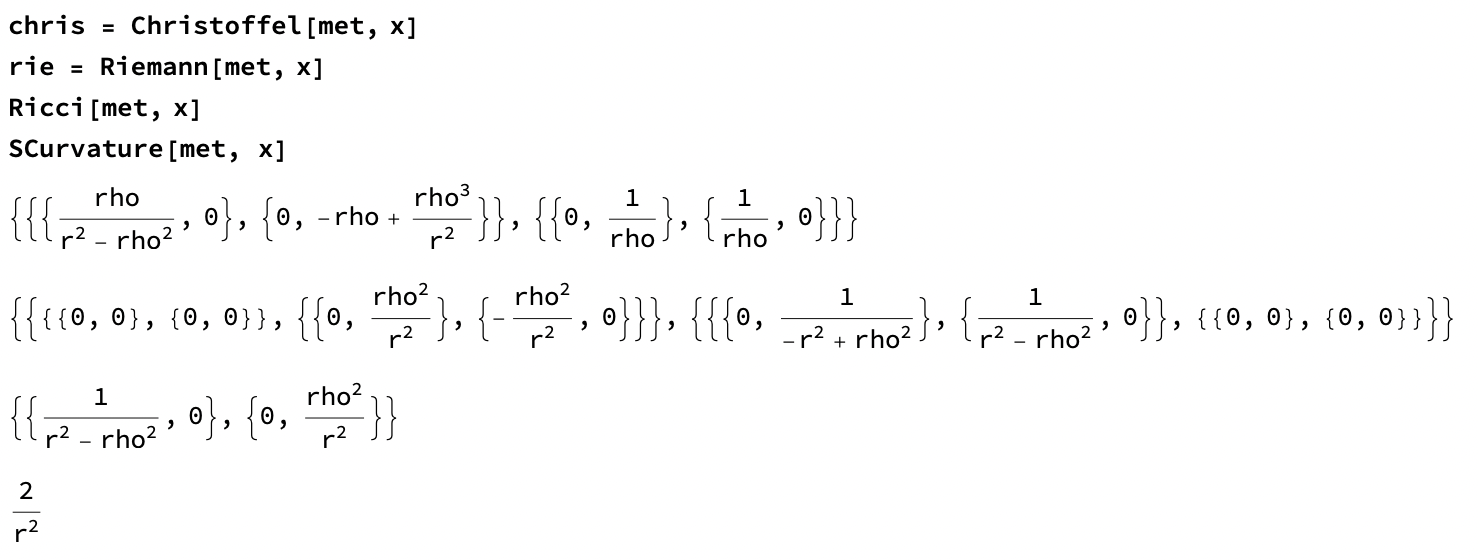
\includegraphics[scale=0.5]{problem2.png}
	\end{center}
\end{solution}

\begin{problem}{3}
Express the gravitational potential $\Phi$ at the surface of the Earth in terms of the mass $M$ and radius $R$ of the Earth. Use this and the result from the geodesic equation derived in lecture to express the metric component $g_{00} = -1 + h_{00}$ in terms of $M$ and $R$. Estimate the numerical value of $h_{00}$ and show how small it is compared to the leading term $-1$.
\end{problem}

\begin{solution}
	The gravitational potential at the surface of the earth is
	\[
		\Phi = -\frac{GM}{R},
	\]
	so by the formulas derived in class, the term $h_{00}$ is
	\[
		h_{00} \approx -\frac{2\Phi}{c^2} = \frac{2GM}{Rc^2} = \frac{2(\Gsi{6.67e-11})(\kgsi{5.972e24})}{(\msi{6.378e6})(\msi{3.00e8})^2}=\psssi{1.39e-9}.
	\]
	This is quite small compared to the leading term $-1$, meaning that spacetime is not that curved at the surface of the Earth.
\end{solution}

\begin{problem}{4}
Prove the following Bianchi identities
\[
	\nabla_\lambda R_{\mu\nu\alpha\beta} + \nabla_\nu R_{\lambda\mu\alpha\beta} + \nabla_\mu R_{\nu\lambda\alpha\beta} = 0.
\]
\end{problem}

\begin{solution}
	First of all, in any associative algebra with commutator $[A, B] = AB-BA$, we have the Jacobi identity
	\[
		\begin{aligned}
			[A, [B,C]] + [B,[C,A]] + [C, [A,B]]
			 & =0  \\
			ABC-ACB - BCA+CBA + BCA-BAC
			-CAB+ACB + CAB - CBA - ABC+BAC
			 & =0. \\
		\end{aligned}
	\]
	Using the identity $[\nabla_{\alpha}, \nabla_\beta] A^\mu = R^\mu_{\lambda\alpha\beta} A^\lambda$, and applying the Jacobi identity, we get
	\[
		\begin{aligned}
			[\nabla_\alpha, [\nabla_\beta, \nabla_\gamma]]A^\mu +
			[\nabla_\beta, [\nabla_\gamma, \nabla_\alpha]]A^\mu +
			[\nabla_\gamma, [\nabla_\alpha, \nabla_\beta]]A^\mu
			  & = 0 \\
			\nabla_\alpha [\nabla_\beta, \nabla_\gamma] A^{\mu} - [\nabla_\beta, \nabla_\gamma]\nabla_\alpha A^{\mu}
			+\nabla_\beta[\nabla_\gamma, \nabla_\alpha] A^{\mu} - [\nabla_\gamma, \nabla_\alpha]\nabla_\beta A^{\mu}
			+\nabla_\gamma[\nabla_\alpha, \nabla_\beta] A^{\mu} - [\nabla_\alpha, \nabla_\beta]\nabla_\gamma A^{\mu}
			  & =0  \\
			\nabla_\alpha R^{\mu}_{\lambda\beta\gamma}A^\lambda
			-R^{\mu}_{\lambda\beta\gamma} \nabla_\alpha A^\lambda
			+\nabla_\beta R^{\mu}_{\lambda\gamma\alpha}A^\lambda
			-R^{\mu}_{\lambda\gamma\alpha} \nabla_\beta A^\lambda
			+\nabla_\gamma R^{\mu}_{\lambda\alpha\beta}A^\lambda
			-R^{\mu}_{\lambda\alpha\beta} \nabla_\gamma A^\lambda
			  & =0  \\
			(
			\nabla_\alpha R^{\mu}_{\lambda\beta\gamma}A^\lambda
			+\nabla_\beta R^{\mu}_{\lambda\gamma\alpha}A^\lambda
			+\nabla_\gamma R^{\mu}_{\lambda\alpha\beta}A^\lambda
			) -
			(
			R^{\mu}_{\lambda\beta\gamma} \nabla_\alpha A^\lambda
			+R^{\mu}_{\lambda\gamma\alpha} \nabla_\beta A^\lambda
			+R^{\mu}_{\lambda\alpha\beta} \nabla_\gamma A^\lambda
			) & =0  \\
			(
			\nabla_\alpha R_{\mu\lambda\beta\gamma}A^\lambda
			+\nabla_\beta R_{\mu\lambda\gamma\alpha}A^\lambda
			+\nabla_\gamma R_{\mu\lambda\alpha\beta}A^\lambda
			) -
			(
			R_{\mu\lambda\beta\gamma} \nabla_\alpha A^\lambda
			+R_{\mu\lambda\gamma\alpha} \nabla_\beta A^\lambda
			+R_{\mu\lambda\alpha\beta} \nabla_\gamma A^\lambda
			) & =0  \\
		\end{aligned}
	\]
	The left side of this difference must be zero by the Bianchi identity proved last time, so we are left with
	\[
		\nabla_\alpha R_{\mu\lambda\beta\gamma}A^\lambda
		+\nabla_\beta R_{\mu\lambda\gamma\alpha}A^\lambda
		+\nabla_\gamma R_{\mu\lambda\alpha\beta}A^\lambda = 0.
	\]
	By the symmetry of the Riemann tensor, we can rearrange this to get
	\[
		(\nabla_\alpha R_{\beta\gamma\mu\lambda}
		+\nabla_\beta R_{\gamma\alpha\mu\lambda}
		+\nabla_\gamma R_{\alpha\beta\mu\lambda})A^\lambda = 0.
	\]
	A similar argument works for higher rank tensor -- for example $[\nabla_\alpha, \nabla_\beta] T^{\mu}_\nu = R^\mu_{\lambda\alpha\beta} T^{\mu}_\nu - R^\lambda_{\mu\beta\gamma} T^{\mu}_{\nu}$ gives the same equations since all involved relations are linear. Since this holds for all tensors, we have
	\[
		\nabla_\alpha R_{\beta\gamma\mu\lambda}
		+\nabla_\beta R_{\gamma\alpha\mu\lambda}
		+\nabla_\gamma R_{\alpha\beta\mu\lambda} = 0.
	\]
\end{solution}

\begin{problem}{5}
The general form for an ``Einstein-like'' equation is
\[
	\mathcal{O}^{\mu\nu} = R^{\mu\nu} + \lambda g^{\mu\nu} R + \Lambda g^{\mu\nu},
\]
where $\lambda$ and $\Lambda$ are constants. Show that if we require that $\nabla_{\mu}\mathcal{O}^{\mu\nu}=0$, the parameter $\lambda=-1/2$ and $\Lambda$ is arbitrary.
\end{problem}

\begin{solution}
	Throughout, let $\nabla_\mu$ be a metric-compatible covariant derivative.
	By the equation, the conservation of the tensor $\mathcal{O}^{\mu\nu}$ becomes
	\[
		\begin{aligned}
			\nabla_\mu \mathcal{O}^{\mu\nu} & = \nabla_\mu R^{\mu\nu} + \nabla_\mu \lambda g^{\mu\nu}R + \nabla_\mu\Lambda g^{\mu\nu}                                                                          \\
			                                & = \nabla_\mu R^{\mu\nu} + \lambda g^{\mu\nu}\nabla_\mu R                                                                                                         \\
			                                & = \nabla_\mu g^{\mu\alpha}g^{\nu\beta}R_{\alpha\beta} + \lambda g^{\mu\nu}\nabla_\mu g^{\alpha\beta}R_{\alpha\beta}                                              \\
			                                & =
			g^{\mu\alpha} g^{\nu\beta} g^{\kappa\rho} \nabla_\mu R_{\kappa\alpha\rho\beta}
			+\lambda g^{\mu\nu}g^{\alpha\beta} g^{\kappa\rho} \nabla_\mu R_{\kappa\alpha\rho\beta}                                                                                                             \\
			                                & = (g^{\mu\alpha}g^{\nu\beta} + \lambda g^{\mu\nu}g^{\alpha\beta}) \nabla_\mu R{_{\kappa\alpha\rho\beta}}\hspace{5em}\textrm{after contracting by }g_{\kappa\rho} \\
		\end{aligned}
	\]
	Next, let's apply $\nabla_\mu$ to the Bianchi identity to get
	\[
		\begin{aligned}
			\nabla_\mu R_{\kappa\alpha\rho\beta} + \nabla_\mu R_{\kappa\beta\alpha\rho} + \nabla_\mu R_{\kappa\rho\beta\alpha}
			                                                              & =0                                                                                    \\
			g^{\mu\alpha} g^{\nu\beta} \nabla_\mu R_{\kappa\alpha\rho\beta} +  g^{\mu\alpha} g^{\nu\beta}  \nabla_\mu R_{\kappa\beta\alpha\rho} + g^{\mu\alpha} g^{\nu\beta} \nabla_\mu R_{\kappa\rho\beta\alpha}
			                                                              & =0 \hspace{3em}\textrm{after contracting by } g_{\mu\alpha}\textrm{ and }g^{\nu\beta} \\
			g^{\mu\alpha} g^{\nu\beta} \nabla_\mu R_{\kappa\alpha\rho\beta}
			- g^{\mu\nu} g^{\alpha\beta} \nabla_\mu R_{\kappa\alpha\rho\beta}
			+ g^{\mu\alpha} g^{\nu\beta} \nabla_\mu R_{\kappa\alpha\rho\beta}
			                                                              & =0 \hspace{3em}\textrm{by (anti)symmetry and renaming variables}                      \\
			g^{\mu\nu}g^{\alpha\beta}\nabla_\mu R_{\kappa\alpha\rho\beta} & = 2g^{\mu\alpha}g^{\nu\beta}\nabla_\mu R_{\kappa\alpha\rho\beta}.
		\end{aligned}
	\]
	Plugging this into the equation we derived earlier involving $\lambda$, it's clear that $\lambda = -1/2$, and so the Einstein equation must take the form
	\[
		\mathcal{O}^{\mu\nu} = R^{\mu\nu} - \frac{1}{2}g^{\mu\nu} R + \Lambda g^{\mu\nu}.
	\]
\end{solution}

\begin{problem}{6}
Remind yourself and briefly outline the steps that have led us to the Einstein equation. At the final step to the explicit form of the Einstein equation, make use of the result shown above.
\end{problem}

\begin{solution}
	One of the consequences of Maxwell's equations is that the speed of light is constant irrespective of the reference frame of an inertial observer. This was one of the motivations which led Einstein to consider special relativity, which postulates that the laws of physics (including constancy of the speed of light) are the same in any inertial reference frame. With some basic thought experiments, we can see some interesting consequences of this additional axiom -- namely that distances, time duration, simultaneity are all observer dependent. These implications are encapsulated by an elegant mathematical object known as the Minkowski metric, which is an inner product on a $4$-dimensional vector space with signature $(1,3)$.

	To address the case of a reference frame which is under the influence of gravity, Einstein noticed that an observer freely falling under the influence of gravity is experiences the same laws of physics as an inertial reference frame. This is a special property of the force of gravity since objects of any mass accelerate the same way under gravitational influence. Similarly, a frame experiencing a uniform gravitational field is equivalent to a frame accelerating at a constant rate. Einstein called this the equivalence principle, and referred to it as his ``happiest thought''. Again, using some basic thought experiments, some implications of this principle can be derived -- for example that light bends towards massive objects, time slows down near massive objects, etc...
	This suggests that gravity ``bends'' spacetime.

	Combined with the ideas of special relativity, it's clear that all of this physics can be modeled by a curved manifold equipped with a Lorentzian metric. The curvature of the manifold corresponds to general relativistic effects, and the metric corresponds to special relativistic effects. Using the geodesic equation, the curvature of this manifold corresponds to the ``force of gravity'' and geodesic paths correspond to the motion of a particle under gravitational influence.

	Recall the Poisson equation from Newtonian mechanics which takes the form
	\[
		\nabla^2 \Phi = 4\pi G \rho.
	\]
	Here $\Phi$ is the gravitational potential, $\rho$ is the mass density. The general equation we come up with should be manifestly covariant under the Lorentz metric in order for it to satisfy relativity -- so it must be phrased in the language of tensor calculus. A natural tensor we could consider is the stress-energy tensor $T^{\mu\nu}$ which is a conserved quantity, i.e. $\nabla_\mu T^{\mu\nu} = 0$. The $T^{00}$ component is exactly equal to $\rho$, so this might lead us to a good generalization of the Poisson equation. The left-hand side should then only contain second-order derivatives in the metric $g$. The general form of such a tensor involves the Riemann curvature tensor, Ricci scalar, and metric itself. Thus, the Einstein equation should have the form
	\[
		R^{\mu\nu} + \lambda g^{\mu\nu} R + \Lambda g^{\mu\nu} = \kappa T^{\mu\nu}.
	\]
	Since both sides must be conserved, the previous problem implies that $\lambda=-1/2$. We call $G^{\mu\nu} = R^{\mu\nu}-g^{\mu\nu}R/2$ the Einstein tensor, and after solving for $\kappa$ using the Poisson equation, the Einstein equation has the form
	\[
		G^{\mu\nu} + \Lambda g^{\mu\nu} = \frac{8\pi G}{c^4}T^{\mu\nu},
	\]
	for $\Lambda$ some constant.
\end{solution}

\begin{problem}{7}
Use the Mathematica code to reproduce the Ricci tensor of the most general, static, spherically symmetric spacetime metric.
\end{problem}

\begin{solution}
	Using the Schwarzchild metric
	\[
		g_{\mu\nu} =
		\left(
		\begin{array}{cccc}
				\frac{2 M}{r}-1 & 0                                 & 0   & 0                   \\
				0               & \left(1-\frac{2 M}{r}\right)^{-1} & 0   & 0                   \\
				0               & 0                                 & r^2 & 0                   \\
				0               & 0                                 & 0   & r^2 \sin ^2(\theta) \\
			\end{array}
		\right),
	\]
	Mathematica gives us the Ricci tensor $R^{\mu\nu}=0$ and $R=0$, proving that this is a solution for the vacuum Einstein equations.
	\begin{center}
		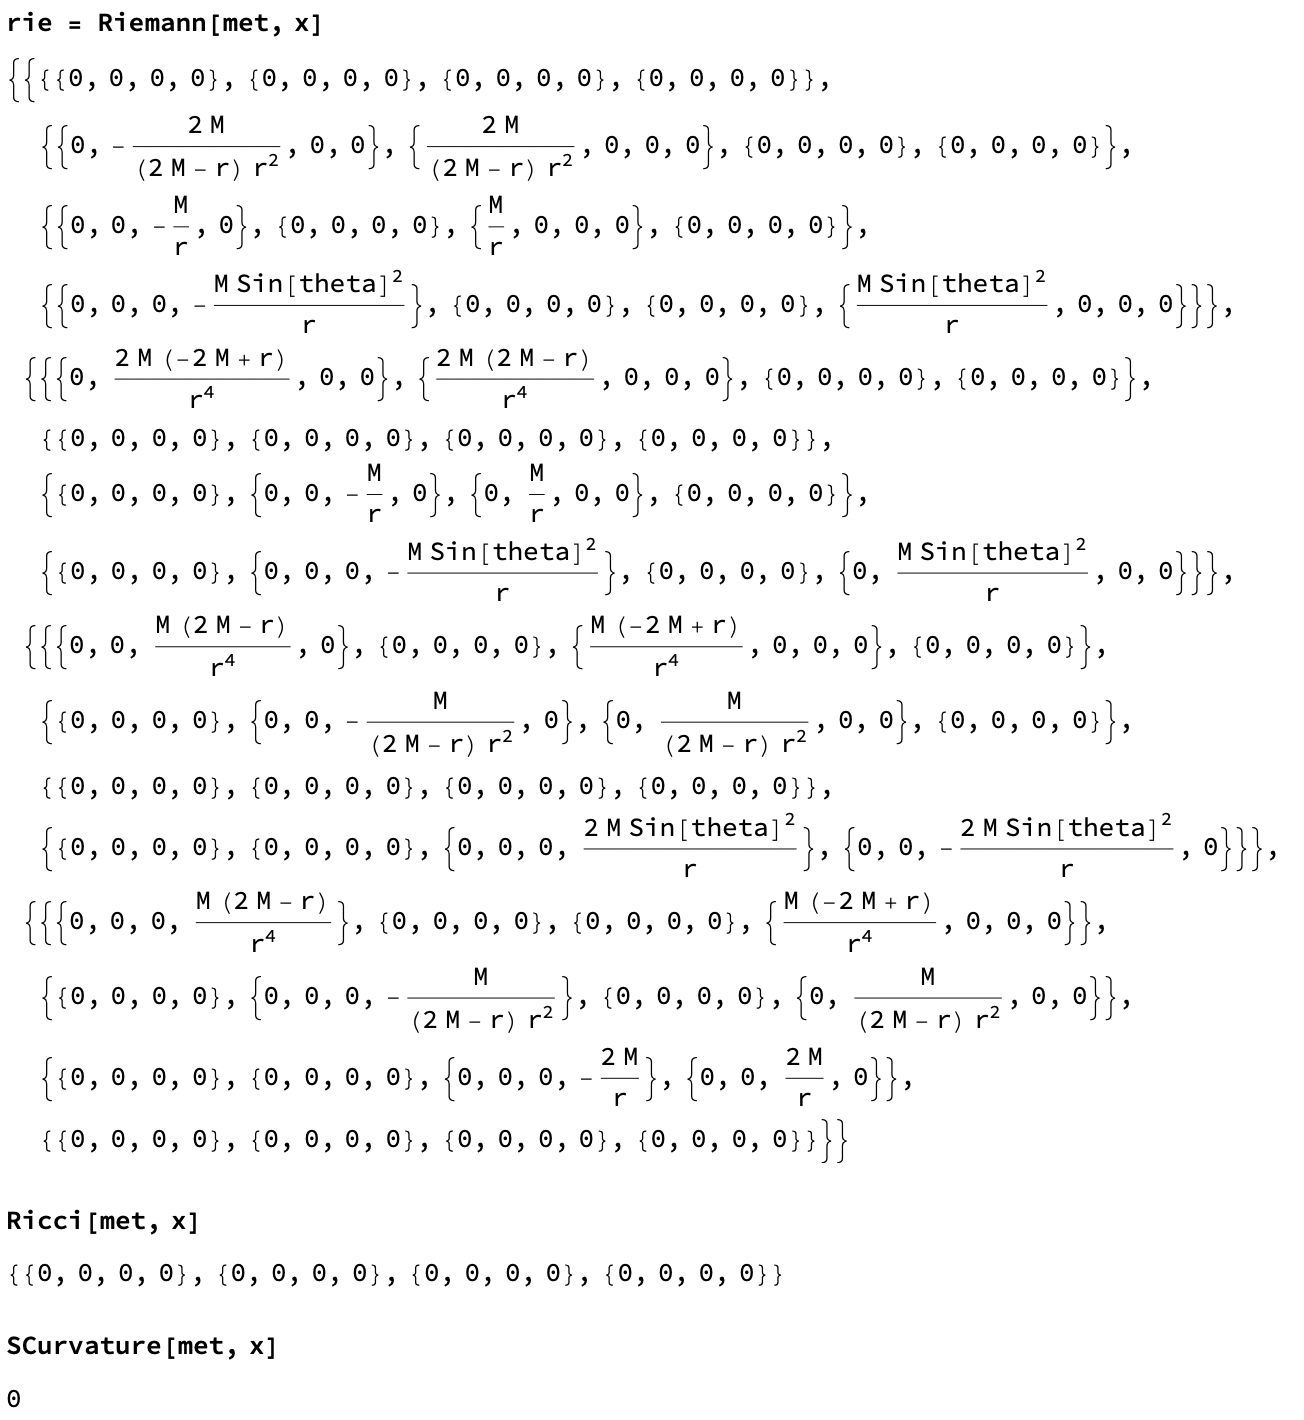
\includegraphics[scale=0.5]{problem7.png}
	\end{center}
\end{solution}

\end{document}
